% -*- Mode:TeX -*-

%% IMPORTANT: The official thesis specifications are available at:
%%            http://libraries.mit.edu/archives/thesis-specs/
%%
%%            Please verify your thesis' formatting and copyright
%%            assignment before submission.  If you notice any
%%            discrepancies between these templates and the 
%%            MIT Libraries' specs, please let us know
%%            by e-mailing thesis@mit.edu

%% The documentclass options along with the pagestyle can be used to generate
%% a technical report, a draft copy, or a regular thesis.  You may need to
%% re-specify the pagestyle after you \include  cover.tex.  For more
%% information, see the first few lines of mitthesis.cls. 

%\documentclass[12pt,vi,twoside]{mitthesis}
%%
%%  If you want your thesis copyright to you instead of MIT, use the
%%  ``vi'' option, as above.
%%
%\documentclass[12pt,twoside,leftblank]{mitthesis}
%%
%% If you want blank pages before new chapters to be labelled ``This
%% Page Intentionally Left Blank'', use the ``leftblank'' option, as
%% above. 

\documentclass[12pt,twoside]{mitthesis}
\usepackage{lgrind}
%% These have been added at the request of the MIT Libraries, because
%% some PDF conversions mess up the ligatures.  -LB, 1/22/2014
\usepackage{cmap}
\usepackage[T1]{fontenc}
\usepackage{hyperref}
\usepackage{listings}
\usepackage{xcolor}

\pagestyle{plain}
\renewcommand{\c}[1]{\texttt{#1}}
\lstset { %
    language=C++,
    backgroundcolor=\color{black!5}, % set backgroundcolor
    basicstyle=\footnotesize,% basic font setting
}


%% This bit allows you to either specify only the files which you wish to
%% process, or `all' to process all files which you \include.
%% Krishna Sethuraman (1990).

%%\typein [\files]{Enter file names to process, (chap1,chap2 ...), or `all' to
%%process all files:}
\def\files{all}
\def\all{all}
\ifx\files\all \typeout{Including all files.} \else \typeout{Including only \files.} \includeonly{\files} \fi

\begin{document}

% -*-latex-*-
% 
% For questions, comments, concerns or complaints:
% thesis@mit.edu
% 
%
% $Log: cover.tex,v $
% Revision 1.8  2008/05/13 15:02:15  jdreed
% Degree month is June, not May.  Added note about prevdegrees.
% Arthur Smith's title updated
%
% Revision 1.7  2001/02/08 18:53:16  boojum
% changed some \newpages to \cleardoublepages
%
% Revision 1.6  1999/10/21 14:49:31  boojum
% changed comment referring to documentstyle
%
% Revision 1.5  1999/10/21 14:39:04  boojum
% *** empty log message ***
%
% Revision 1.4  1997/04/18  17:54:10  othomas
% added page numbers on abstract and cover, and made 1 abstract
% page the default rather than 2.  (anne hunter tells me this
% is the new institute standard.)
%
% Revision 1.4  1997/04/18  17:54:10  othomas
% added page numbers on abstract and cover, and made 1 abstract
% page the default rather than 2.  (anne hunter tells me this
% is the new institute standard.)
%
% Revision 1.3  93/05/17  17:06:29  starflt
% Added acknowledgements section (suggested by tompalka)
% 
% Revision 1.2  92/04/22  13:13:13  epeisach
% Fixes for 1991 course 6 requirements
% Phrase "and to grant others the right to do so" has been added to 
% permission clause
% Second copy of abstract is not counted as separate pages so numbering works
% out
% 
% Revision 1.1  92/04/22  13:08:20  epeisach

% NOTE:
% These templates make an effort to conform to the MIT Thesis specifications,
% however the specifications can change.  We recommend that you verify the
% layout of your title page with your thesis advisor and/or the MIT 
% Libraries before printing your final copy.
\title{Pinky: Interactively Analyzing Large EEG Datasets}

\author{Joshua Blum}
% If you wish to list your previous degrees on the cover page, use the 
% previous degrees command:
%       \prevdegrees{A.A., Harvard University (1985)}
% You can use the \\ command to list multiple previous degrees
%       \prevdegrees{B.S., University of California (1978) \\
%                    S.M., Massachusetts Institute of Technology (1981)}
\department{Department of Electrical Engineering and Computer Science}

% If the thesis is for two degrees simultaneously, list them both
% separated by \and like this:
% \degree{Doctor of Philosophy \and Master of Science}
\degree{Master of Engineering in Computer Science and Engineering}

% As of the 2007-08 academic year, valid degree months are September, 
% February, or June.  The default is June.
\degreemonth{February}
\degreeyear{2016}
\thesisdate{January 04, 2016}

%% By default, the thesis will be copyrighted to MIT.  If you need to copyright
%% the thesis to yourself, just specify the `vi' documentclass option.  If for
%% some reason you want to exactly specify the copyright notice text, you can
%% use the \copyrightnoticetext command.  
%\copyrightnoticetext{\copyright IBM, 1990.  Do not open till Xmas.}

% If there is more than one supervisor, use the \supervisor command
% once for each.
\supervisor{Prof. Samuel Madden}

% This is the department committee chairman, not the thesis committee
% chairman.  You should replace this with your Department's Committee
% Chairman.
\chairman{Dr. Christopher Terman}{Chairman, Masters of Engineering Thesis Committee}

% Make the titlepage based on the above information.  If you need
% something special and can't use the standard form, you can specify
% the exact text of the titlepage yourself.  Put it in a titlepage
% environment and leave blank lines where you want vertical space.
% The spaces will be adjusted to fill the entire page.  The dotted
% lines for the signatures are made with the \signature command.
\maketitle

% The abstractpage environment sets up everything on the page except
% the text itself.  The title and other header material are put at the
% top of the page, and the supervisors are listed at the bottom.  A
% new page is begun both before and after.  Of course, an abstract may
% be more than one page itself.  If you need more control over the
% format of the page, you can use the abstract environment, which puts
% the word "Abstract" at the beginning and single spaces its text.

%% You can either \input (*not* \include) your abstract file, or you can put
%% the text of the abstract directly between the \begin{abstractpage} and
%% \end{abstractpage} commands.

% First copy: start a new page, and save the page number.
\cleardoublepage
% Uncomment the next line if you do NOT want a page number on your
% abstract and acknowledgments pages.
% \pagestyle{empty}
\setcounter{savepage}{\thepage}
\begin{abstractpage}
% $Log: abstract.tex,v $
% Revision 1.1  93/05/14  14:56:25  starflt
% Initial revision
% 
% Revision 1.1  90/05/04  10:41:01  lwvanels
% Initial revision
% 
%
%% The text of your abstract and nothing else (other than comments) goes here.
%% It will be single-spaced and the rest of the text that is supposed to go on
%% the abstract page will be generated by the abstractpage environment.  This
%% file should be \input (not \include 'd) from cover.tex.

In this thesis, I describe a system I designed and implemented for
interactively analyzing large electroencephalogram (EEG) datasets. Trained
experts, known as encephalographers, analyze EEG data to determine if a patient
has experienced an epileptic seizure. Since EEG analysis is time intensive for
large datasets, there is a growing corpus of unanalyzed EEG data. Fast analysis
is essential for building a set of example data of EEG results, allowing
doctors to quickly classify the behavior of future EEG scans.  My system aims
to reduce the cost of analysis by providing near real-time interaction with the
datasets. The system has three optimized layers handling the storage,
computation, and visualization of the data. I evaluate the design choices for
each layer and compare three different implementations across different
workloads.

\end{abstractpage}

% Additional copy: start a new page, and reset the page number.  This way,
% the second copy of the abstract is not counted as separate pages.
% Uncomment the next 6 lines if you need two copies of the abstract
% page.
% \setcounter{page}{\thesavepage}
% \begin{abstractpage}
% % $Log: abstract.tex,v $
% Revision 1.1  93/05/14  14:56:25  starflt
% Initial revision
% 
% Revision 1.1  90/05/04  10:41:01  lwvanels
% Initial revision
% 
%
%% The text of your abstract and nothing else (other than comments) goes here.
%% It will be single-spaced and the rest of the text that is supposed to go on
%% the abstract page will be generated by the abstractpage environment.  This
%% file should be \input (not \include 'd) from cover.tex.

In this thesis, I describe a system I designed and implemented for
interactively analyzing large electroencephalogram (EEG) datasets. Trained
experts, known as encephalographers, analyze EEG data to determine if a patient
has experienced an epileptic seizure. Since EEG analysis is time intensive for
large datasets, there is a growing corpus of unanalyzed EEG data. Fast analysis
is essential for building a set of example data of EEG results, allowing
doctors to quickly classify the behavior of future EEG scans.  My system aims
to reduce the cost of analysis by providing near real-time interaction with the
datasets. The system has three optimized layers handling the storage,
computation, and visualization of the data. I evaluate the design choices for
each layer and compare three different implementations across different
workloads.

% \end{abstractpage}

\cleardoublepage

\section*{Acknowledgments}

This is the acknowledgements section.  You should replace this with your
own acknowledgements.

%%%%%%%%%%%%%%%%%%%%%%%%%%%%%%%%%%%%%%%%%%%%%%%%%%%%%%%%%%%%%%%%%%%%%%
% -*-latex-*-

% Some departments (e.g. 5) require an additional signature page.  See
% signature.tex for more information and uncomment the following line if
% applicable.
% % -*- Mode:TeX -*-
%
% Some departments (e.g. Chemistry) require an additional cover page
% with signatures of the thesis committee.  Please check with your
% thesis advisor or other appropriate person to determine if such a 
% page is required for your thesis.  
%
% If you choose not to use the "titlepage" environment, a \newpage
% commands, and several \vspace{\fill} commands may be necessary to
% achieve the required spacing.  The \signature command is defined in
% the "mitthesis" class
%
% The following sample appears courtesy of Ben Kaduk <kaduk@mit.edu> and
% was used in his June 2012 doctoral thesis in Chemistry. 

\begin{titlepage}
\begin{large}
This doctoral thesis has been examined by a Committee of the Department
of Chemistry as follows:

\signature{Professor Jianshu Cao}{Chairman, Thesis Committee \\
   Professor of Chemistry}

\signature{Professor Troy Van Voorhis}{Thesis Supervisor \\
   Associate Professor of Chemistry}

\signature{Professor Robert W. Field}{Member, Thesis Committee \\
   Haslam and Dewey Professor of Chemistry}
\end{large}
\end{titlepage}


\pagestyle{plain}
  % -*- Mode:TeX -*-
%% This file simply contains the commands that actually generate the table of
%% contents and lists of figures and tables.  You can omit any or all of
%% these files by simply taking out the appropriate command.  For more
%% information on these files, see appendix C.3.3 of the LaTeX manual.
\tableofcontents
\newpage
\listoffigures
\newpage
\listoftables


%% This is an example first chapter.  You should put chapter/appendix that you
%% write into a separate file, and add a line \include{yourfilename} to
%% main.tex, where `yourfilename.tex' is the name of the chapter/appendix file.
%% You can process specific files by typing their names in at the 
%% \files=
%% prompt when you run the file main.tex through LaTeX.
\chapter{Introduction}\label{intro-ch}

Many applications require a domain expert to visually inspect and process a
dataset on a stream of incoming data. The problem with such manual inspection
is it's inability to scale as datasets grow exponentially \cite{exp-growth}. As
the data set grows, it becomes difficult to visualize and interact with
\cite{immens} and there are also many cases of false positives which the expert
should not have to manually reclassify. We with to focus on the field of
medical data, where doctors have to view a patient's data and extract relevant
information for treatment. Specifically, we focus on electroencephalogram (EEG)
readings, a test which is used to detect abnormalities related to the
electrical activity of the brain. \\

Today, doctors are faced with having to store large amounts of patient data
without analysis since they lack the tools to efficiently view datasets are a
large scale. To remedy this, we have designed and implemented a system, Pinky,
which can process large amounts of EEG data, allowing near real-time
interaction for analysis.


\section{Pinky}

Pinky is a doctor's newest tool for analysing the brain, see Figure
\ref{fig:pinky-and-the-brain}. Working with a team of researchers at
Massachusetts General Hospital, we have designed and implemented the system to
handle the fast growing corpus of EEG data that is being collected. This
end-to-end system handles the storage, computation, and visualization of EEG.
The goal of the system is to provide a scalable architecture for concurrent
analysis of patient records with near real time interactivity. Each layer of
the system has been optimized for use and evaluated across hundreds of GB of
patient data. \\

\begin{figure}[h]
\begin{center}
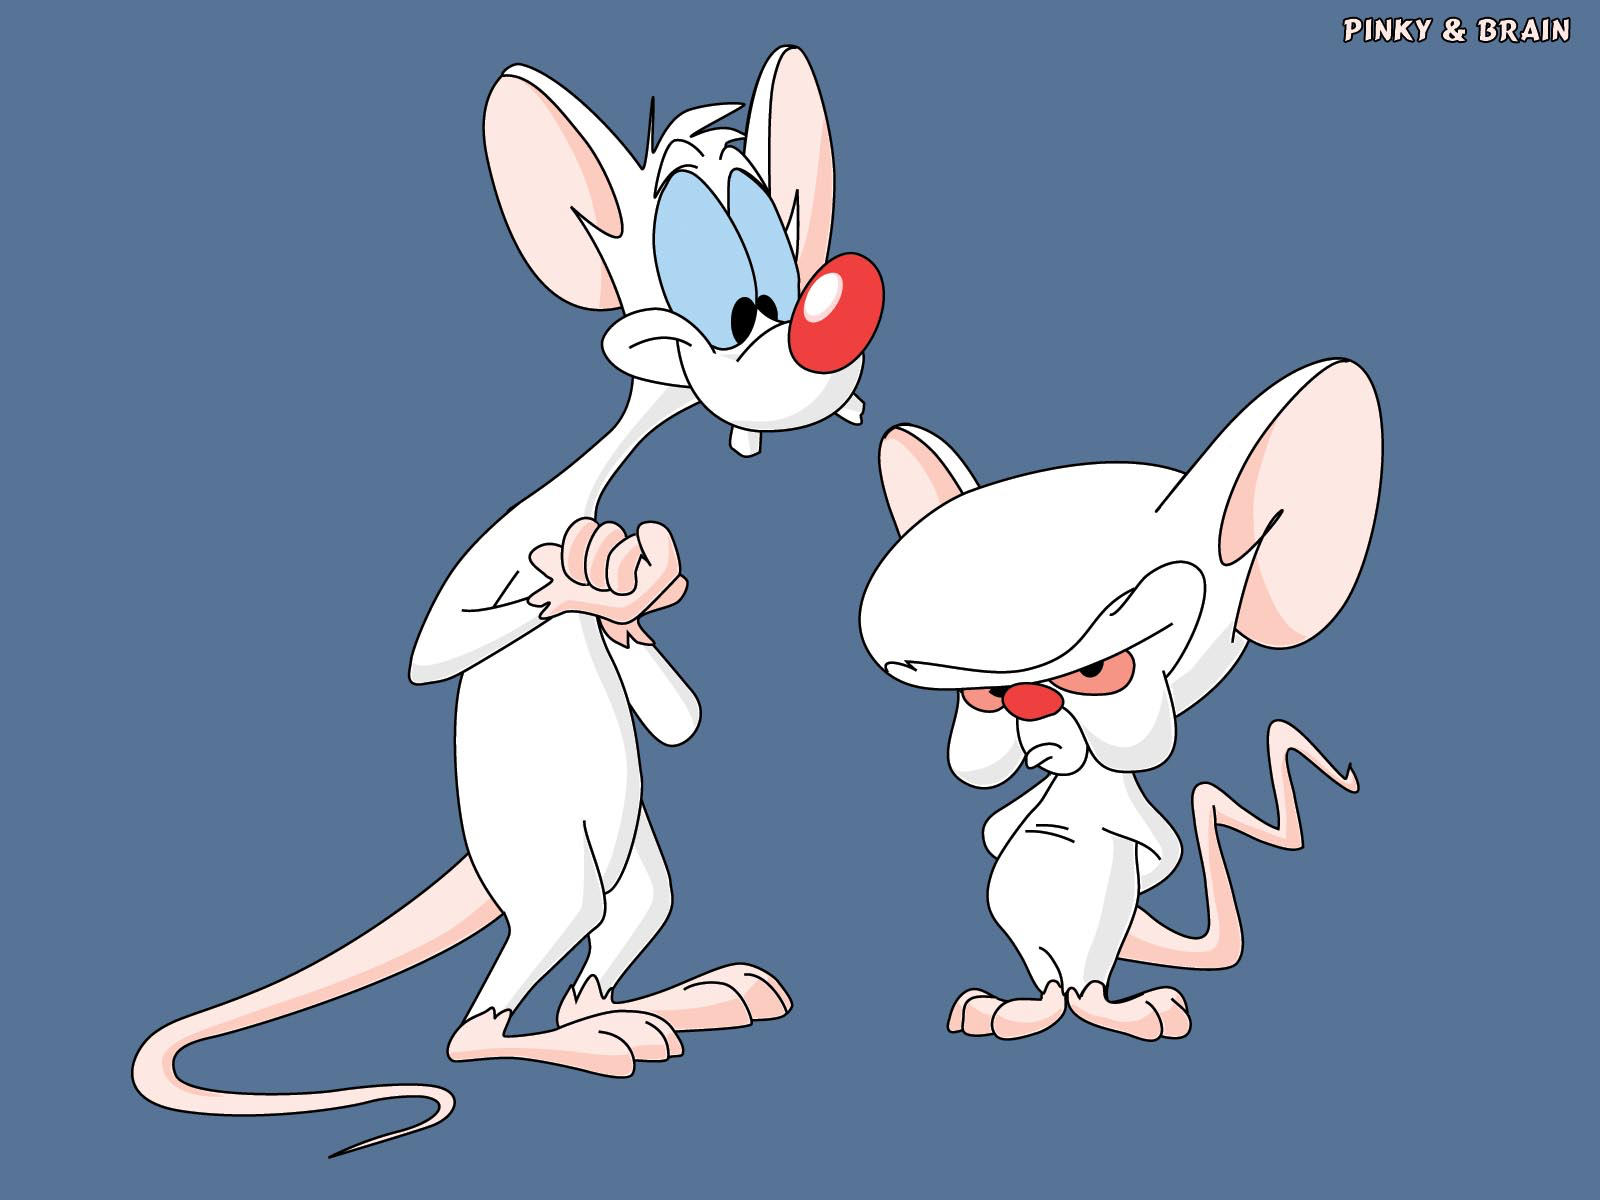
\includegraphics[scale=0.5]{./img/pinky-and-the-brain.png}
\caption{Etymology of Pinky's name.}
\label{fig:pinky-and-the-brain}
\end{center}
\end{figure}

\section{Overview of EEG Analysis}

TODO:
What is EEG analysis? Why is it important? What is the scale of the problem? How have we fixed it?

\section{System Architecture}

The system is comprised of three coupled layers which handle, storage,
computation and visualization. Figure \ref{fig:system-architecture} shows the
overall architecture of the system.

\begin{figure}[h]
\begin{center}
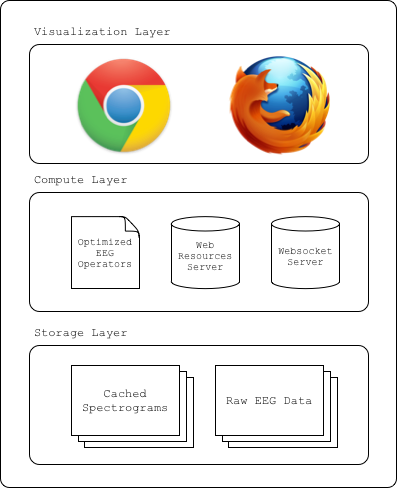
\includegraphics[scale=0.75]{./img/system-architecture.png}
\caption{Pinky System Architecture.}
\label{fig:system-architecture}
\end{center}
\end{figure}

\subsection{Storage Layer}

The storage layer, discuss in detail in chapter \ref{storage-ch}, is responsible for
storing raw EEG patient data and a copy of the calculated spectrogram. This
datastore must be optimized for both reads and writes of array based data for
multidimensional arrays on the order to tens to hundreds of GB.

\subsection{Compute Layer}

The compute layer, discuss in detail in chapter \ref{compute-ch}, is meant to be an
extendible module which handles the algorithms to calculate the spectrogram and
other EEG related calculations. As we discuss in \ref{discuss-ch:future-work},
there are several extensions the project can take, thus it is important that an
interested developer can easily add functionality to this layer. In addition,
the compute layer contains two servers, one to server the array based data,
interfacing with the optimized EEG algorithms, and a lightweight server for the
web resources to be served to the visualization layer.

\subsection{Visualization Layer}

The visualization layer, discussed in detail in chapter \ref{viz-ch}, is a browser
based module that renders the data to the client. The interface allows users to
query based on a patient's id (medical record number, \c{mrn}) and view a spectrogram
for a given time interval.

\subsection{Visgoth System}

Since enabling interactivity is an important design criteria, we have designed
and built a optimization module for time series visualization in the browser,
Visgoth. This is discussed in detail in chapter \ref{visgoth-ch}.

\section{Usage}

The project code base is available publicly on Github \cite{github}
\url{https://github.com/joshblum/eeg-toolkit} with documentation for installing
the project for development. In addition, we have created Docker \cite{docker}
images that can easily be install for production use. Armed with a dataset, any
curious doctor should be able to install the images and load the data for
analysis. The docker images are available for public use here:
\url{https://hub.docker.com/r/joshblum/eeg-toolkit-webapp} and
\url{https://hub.docker.com/r/joshblum/eeg-toolkit-toolkit}. Specific
installation instructions can be found with the github project.

\section{Contributions}

Pinky make several contributions:

\begin{itemize}
  \item Implements an abstraction for array based storage systems.
  \item Implements 4 different backends to adhere to the abstraction.
  \item Evaluates the different backends for multiple input ranges and workloads.
  \item Implements optimized algorithms for analysing EEG data.
  \item Provides an extendible framework for accessing array based data and visualizing it in the browser.
  \item Implements scalable in-browser visualizations using the client's GPU.
  \item Implements a new system, Visgoth, for reducing latency for time series based visualizations.
\end{itemize}

These contributions enable doctors and medical expert analysts to interactively
analyse EEG data at scale.


\chapter{Storage Layer}\label{storage-ch}

Pinky stores both raw EEG voltage readings and calculated spectrograms. The raw
EEG data is simply a matrix with a column for each sensor (see
Figure~\ref{fig:electrodes}) and a data sample read by the sensor at each row.
Similarly, we store the spectrogram, a range of frequencies across time, as a
multidimensional array. Since matrices of floating point values represent both
raw EEG data and the spectrogram visualization, the system requires an
efficient way to store and query such large multidimensional arrays. The
storage layer meets this requirement by providing an abstraction called the
\c{StorageBackend} for storing array based data. The abstraction gives read and
write access to 2-dimensional matrices of \c{float} values. Since the
interactivity the system demands requires efficient querying of the data, we
evaluate different array based storage systems and compare the tradeoffs of
each against a simple storage system that we implement.

\section{Design}

The \c{StorageBackend} abstraction provides a thin layer over existing array
based storage systems to provide a consistent API for evaluation across
different systems. The goal is to efficiently expose read and write access to
large array based datasets. A patient EEG scan typically lasts 24 hours, but
can run for up 7 days \cite{ceeg-3}. The raw output of voltage readings yield a
file from tens to hundreds of gigabytes in size. We assume that the entire
dataset cannot always fit into the memory of the server, given that it must
concurrently respond to multiple client queries. Thus, the \c{StorageBackend}
should rely on maintaining an efficient on disk representation of the data. \\

A \c{StorageBackend} implementation must primarily handle three different
workloads. The first is data ingestion. This is a write heavy workload --
reading patient data files from disk and storing them in the system. Secondly,
spectrogram data is typically written once in a precomputation step, and saved
for later analysis. This workload is primarily read heavy, since the computed
spectrogram is much smaller in size than the raw input file.  After being
stored, efficient reads are required for an analyst to access the
visualizations.

\subsection{Ingestion Workload}

Once a patient scan is complete, the system ingests the raw data file for
analysis. The raw data is initially stored in the European Data Format (EDF)
\cite{edf}, a simple binary format for storing multichannel biological and
physical signals. During ingestion, we read the data in chunks of configurable
size from an input EDF file and convert them for storage within the system.
This workload requires the storage system to efficiently handle the addition of
large datasets. We evaluate the performance when ingesting data in
Section~\ref{storage-ch:ingestion-exp}.

\subsection{Precomputation Workload}

After ingesting a file into the system, the spectrogram for a patient is
computed, reading the raw values from the storage system. This precomputation
step is important for minimizing the latency when serving the visualization.
The precomputation calculation involves reading columns of the raw data to
perform the spectrogram calculation and writing the spectrogram matrix back to
the datastore. We describe the details of the calculation in
Section~\ref{compute-ch:design-spectrogram}. This workload requires efficient
reading of individual columns in the raw data and, similarly to the ingestion
workload, the ability to write dense matrices efficiently.

\subsection{Visualization Serving Workload}

In practice, the primary workload the storage system must handle is serving
chunks of a calculated visualization. Analysts will request data for a given
patient and time interval and need to be able to quickly have the results
rendered. This workload requires efficient reading of chunks of the matrix.

\section{Implementation}

The storage layer is implemented in C++, providing a common interface to access
array based datasets. We create a \c{StorageBackend} by inheriting from the
\c{AbstractStorageBackend} interface and implementing the methods described in
Section~\ref{storage-ch:api} using an array storage system. This design allows
us to interchange storage systems for evaluation without affecting other layers
within the overall system. To compare the tradeoffs between different array
store systems for each workload, we implement 3 versions of \c{StorageBackend}
using two existing systems, HDF5 \cite{hdf5} and TileDB \cite{tiledb} and our
own implementation as a baseline. \\

We begin by describing the API in Section~\ref{storage-ch:api} followed by a
description of each implementation in
~\cref{storage-ch:implementation-binary,storage-ch:implementation-hdf5,storage-ch:implementation-tiledb}.
The command line programs that are available for this layer are described in
Section~\ref{storage-ch:implementation-cmd}, and finally we discuss some
overall optimizations in Section~\ref{storage-ch:opt}.

\subsection{StorageBackend API}\label{storage-ch:api}

The \c{StorageBackend} API allows creating, reading, and writing arrays. Each
array corresponds to a patient's unique medical record number, their \c{mrn}.
The API is as follows:

\begin{lstlisting}
    ArrayMetadata get_array_metadata(string mrn);
    void create_array(string mrn, ArrayMetadata* metadata);
    void open_array(string mrn);
    void read_array(string mrn, int ch, int start_offset,
                    int end_offset, float* buf);
    void write_array(string mrn, int ch, int start_offset,
                    int end_offset, float* buf);
    void close_array(string mrn);
\end{lstlisting}

\subsubsection{\c{ArrayMetadata get\_array\_metadata(string mrn)}}

Each array has an associated \c{ArrayMetadata} object which describes the size
of the matrix. Specifically, \c{ArrayMetadata} stores three \c{int} values which
are necessary for the spectrogram calculation and for the client to prepare the
visualization. The values are as follows:

\begin{lstlisting}
    int fs;
    int nrows;
    int ncols;
\end{lstlisting}

\c{fs} is the frequency rate at which the sampling occurred during the EEG
scan. \c{nrows} and \c{ncols} represent the number of rows and columns in the
matrix respectively. Each array based system has a different way of storing
metadata values, thus the \c{ArrayMetadata} object provides a common interface
to access and deserialize them.

\subsubsection{\c{void create\_array(string mrn, ArrayMetadata* metadata);}}

The \c{create\_array} function takes as input a patient's medical record
number, \c{mrn} and a pointer to a \c{ArrayMetadata} object. The function is
responsible for defining the array and persisting the \c{ArrayMetadata} to
disk.

\subsubsection{\c{void open\_array(string mrn);}}

The \c{open\_array} function prepares an array for reading or writing. This
function typically caches certain values for more optimized used. Value caching is
discussed further in Section~\ref{storage-ch:opt}.

\subsubsection{\c{void read\_array(string mrn, int ch, int start\_offset, int end\_offset, float* buf);}}

\c{read\_array} takes in a channel (column) to read, \c{ch}, and a
\c{start\_offset} and \c{end\_offset} describing the subset of rows to
retrieve. When requesting raw EEG data, a single column is passed in. When
requesting a spectrogram, a special channel value \c{ALL} is given since we
want to retrieve all columns for a given time range. We store data values into
the provided buffer \c{buf}.

\subsubsection{\c{void write\_array(string mrn, int ch, int start\_offset, int end\_offset, float* buf);}}

Similarly to \c{read\_array}, \c{write\_array} writes the given column \c{ch}
beginning at \c{start\_offset} and ending at \c{end\_offset} with the values
written from the buffer \c{buf}.

\subsubsection{\c{void close\_array(string mrn);}}

\c{close\_array} frees any cached values for the given \c{mrn} and releases any
other cached resources back to the storage system.

\subsection{EDFBackend}

The \c{EDFBackend} is a \textbf{read-only} implementation of the \c{StorageBackend}
interface. This provides easy access for testing other parts of the system and
conversion between backend types. The backend uses an existing EDF library
implementation \cite{edflib} to read given EDF files. This backend is not
included in the evaluation since the ingestion cost is zero and the
visualizations are not stored in the EDF format.

\subsection{BinaryBackend}\label{storage-ch:implementation-binary}

The \c{BinaryBackend}, inspired by the EDF format, is used as a baseline
against other implementations. We use this as the baseline since the format was
designed to meet the workload requirements and is not a general array storage
system. Comparing the performance of other systems to the \c{BinaryBackend}
allows us to see the overhead a more general purpose system incurs. \\

We use a simple on disk representation for the \c{BinaryBackend}. As
Figure~\ref{fig:binary-bytearray} shows, the first byte of the file contains a
\c{uint32\_t}, containing the length of the header information, $n$. The
following $n$ bytes contain a JSON encoded string with the \c{ArrayMetadata}
information. Following this, we write the array to disk in column-major order
for efficient read access. Since the dataset is dense and the number of rows
are known in advance (\c{nrows}), simple offset calculations determine the
location to read or write the file. \\

\begin{figure}[h]
\begin{center}
\begin{bytefield}{32}
\begin{rightwordgroup}{Header}
  \begin{leftwordgroup}{Header Length}
  \bitbox{4}{43}
  \bitbox{28}{\{"fs": 256,}
  \end{leftwordgroup} \\
  \wordbox{1}{"ncols": 16, "nrows": 15625000\}}
\end{rightwordgroup} \\
\wordbox{1}{column 0} \\
\wordbox{1}{column 1} \\
\wordbox{2}{...} \\
\wordbox{1}{column n}
\end{bytefield}
\caption{On disk data layout for the \c{BinaryBackend} implementation.}
\label{fig:binary-bytearray}
\end{center}
\end{figure}

When performing multiple I/O operations consecutively, for example, writing a
file out in chunks, this implementation suffers from multiple disk seeks. Each
time we perform a read or write operation, the file is opened, we seek to the
appropriate location and finally close the file. To amortize the cost of disk
seeks, we increase the size of the data chunks we read or write.

\subsection{HDF5Backend}\label{storage-ch:implementation-hdf5}

The \c{HDF5Backend} uses the Hierarchical Data Format (HDF) version 5
\cite{hdf5} to store the data. HDF5 is an open source `technology suite' which
meets the requirements for storage for our system. HDF5 is capable of
supporting diverse datasets at scale, fitting the array based model of our
EEG data nicely. \\

Integrating HDF5 as a \c{StorageBackend} is straightforward. Using the HDF5 C++
bindings, we wrap the library calls to read and write data without API methods.
HDF5 has it's own metadata storage which we utilize for keeping the
\c{ArrayMetadata}. One interesting note is in HDF5 you must specify if the
array will read or write the data in chunks, so that the system can layout the
data in the chunk sizes you specify. Our initial implementation left this
detail out, resulting in a 2x cost in performance.

\subsection{TileDBBackend}\label{storage-ch:implementation-tiledb}

TileDB \cite{tiledb} is an ongoing research project by Intel Labs. TileDB
specializes in storing sparse arrays, offering scalable and efficient access to
these datasets. An input dataset can be an arbitrary multidimensional array,
again fitting out model for a storage system. Although our datasets are dense,
we wanted to investigate the performance of TileDB for dense datasets and see
if it can compete with a more mature project such as HDF5.\\

TileDB offers a C API in a shared object library which we use to create the
\c{TileDBBackend}. At the time of writing the project does not yet support
metadata, so we store the \c{ArrayMetadata} as JSON data in a separate file. \\

\subsection{Command Line Programs}\label{storage-ch:implementation-cmd}

The storage layer offers two command line programs \c{edf\_converter <mrn>},
\c{data\_to\_file <mrn> <type>}. The \c{edf\_converter} program takes a \c{mrn}
as input and converts it to the appropriate \c{StorageBackend} format. The
\c{data\_to\_file} program is used to serialize data from a \c{StorageBackend}
to CSV or binary output. These programs are used extensively for testing,
ingestion, and evaluation.

\subsection{Optimizations}\label{storage-ch:opt}

When designing the \c{AbstractStorageBackend}, performance was an important
factor. Internally, we allow child classes to specify a template type \c{T} as
a cache value and also store a mapping from \c{mrn} to \c{ArrayMetadata}. The
goal is to allow each implementation to store some basic information in memory
rather than having to continually fetch from disk. For example, by calling 
\c{open\_array}, we cache objects related to the array for future
use until a call to \c{close\_array}. This allows us to keep a consistent
external API and internally manage access to each library efficiently.

\section{Evaluation}\label{storage-ch:evaluation}

We evaluate the performance of the different \c{StorageBackend} implementations
by testing measuring the time taken to perform file ingestions (described in
Section~\ref{storage-ch:ingestion-exp}) and spectrogram precomputation
(described in Section~\ref{storage-ch:precompute-exp}). All of these
experiments ran on the CSAIL OpenStack infrastructure. We allocated three
instances on `isolated' hosts, where the virtual machine runs using an actual
hardware thread. Each machine had 4 cores available with 8GB of RAM and Intel
Xeon 2.27GHz processors running Ubuntu 14.03.04. Each machine had 330GB of disk
space available for the calculations. To reduce variability between
experiments, each experiment was run a total of 3 times, once on each machine.
Between experiment runs, we clear the file system cache to reduce variations
from caching. \\

These two use cases were chosen since they are the primary workloads of the
system and we want to understand how the different implementations perform for
varying input sizes.\\

The source code and necessary scripts to run the experiments are available
in the project repository \cite{eeg-toolkit}. The repository contains
instructions for building the project and importing a dataset for testing.

\subsection{Ingestion Experiment}\label{storage-ch:ingestion-exp}

The ingestion experiment takes an EDF file and converts it to the appropriate
\c{StorageBackend} format. In the MGH corpus, the largest EDF file is 150GB and
files commonly range from 5GB to 20GB. Thus, to understand how the different
implementations would scale, we use files from 1GB to 128GB in size, varying by
powers of 2, for the experiment. In addition to varying the file size, we also
vary the chunk size read and write with. To reduce system memory consumption we
varied chunk sizes by powers of 2 from 64MB to 128MB. Experimentally, we found
that a chunk size of 256MB was optimal across the file sizes, thus we evaluate
the different backends with this chunk size.

\begin{figure}[h]
\begin{center}
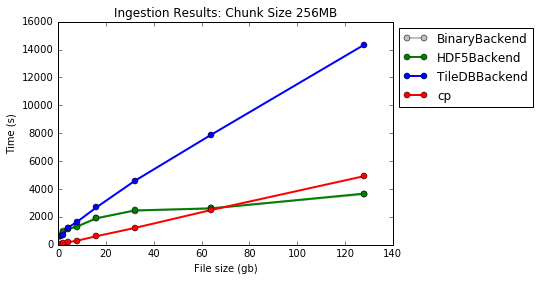
\includegraphics[scale=.75]{./img/ingestion-exp.png}
\caption{Total runtime for different backend implementations in the ingestion
  experiment.}
\label{fig:ingestion-exp}
\end{center}
\end{figure}

As Figure~\ref{fig:ingestion-exp} shows, the \c{HDF5Backend} and
\c{BinaryBackend} scale much more efficiently than the \c{TileDBBackend}. Since
the ingestion experiment is a write heavy workload, the figure shows both the
overall performance as file size increases and speed of writes in the system.
Since the \c{TileDBBackend} scales linearly with the file size, we assume that writes
in this system are much more expensive than the others. \\

When writing the \c{TileDBBackend}, we optimized writes by writing the data in
sorted order. If the data is unsorted, TileDB will internally sort the dataset,
thus we want to avoid incurring this overhead during writes. The only other
clues for the large performance gap would be that the data ingested is dense
and not sparse data, which TileDB is optimized for.

\subsection{Precompute Experiment}\label{storage-ch:precompute-exp}

The precomputation experiment calculates the spectrogram for a given \c{mrn} We
use the same file sizes as in the ingestion experiment, using the ingested data
for this calculation of the spectrogram. Similarly to the ingestion experiment,
we vary the chunk sizes for writing the spectrogram back to the
\c{StorageBackend}. In the evaluation, we use the same chunk size as the
ingestion experiment, 256MB. \\

For this experiment, we evaluate the read time, write time, and total time
across the different \c{StorageBackend} implementations. The read time is
calculated as the sum of all reads across regions when producing the
spectrogram. Similarly, the write time is compute as the total time to write
the calculated spectrogram values across all regions. The total time accounts
for the read and write times in addition to the FFT calculation for computing
the spectrogram.

\subsubsection{Read Time}

\begin{figure}[h]
\begin{center}
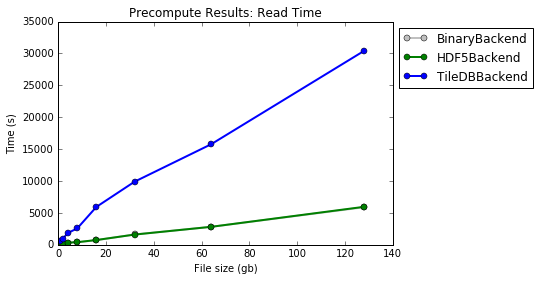
\includegraphics[scale=0.75]{./img/precompute-exp-read-time.png}
\caption{Total read time for different backend implementations in the
  precompute experiment.}
\label{fig:precompute-exp-read-time}
\end{center}
\end{figure}

As Figure~\ref{fig:precompute-exp-read-time} shows, both the \c{BinaryBackend}
and \c{HDF5Backend} have similar read times, with a near constant value
across file sizes. The \c{TileDBBackend} on the otherhand has a growing read
time between processing 32GB and 128GB files. The runtime for the
\c{TileDBackend} is also an order of magnitude greater than the other systems. \\

One possibility for the large performance gap here could be the way TileDB
internally reads data from the disk. The \c{BinaryBackend} takes the entire
memory chunk it reads and interprets it as an array of \c{float} values. Given
the performance similarity to the \c{HDF5Backend}, we can assume a similar
computation is done when extracting data from HDF5. TileDB on the otherhand
reads each cell from memory and converts it to a floating point value. This
pass over the memory manually converting each time could be one reason for the
poor read performance.

\subsubsection{Write Time}

\begin{figure}[h]
\begin{center}
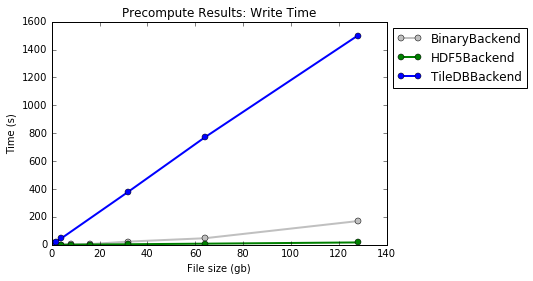
\includegraphics[scale=0.75]{./img/precompute-exp-write-time.png}
\caption{Total write time for different backend implementations in the
  precompute experiment.}
\label{fig:precompute-exp-write-time}
\end{center}
\end{figure}

Similar to Figure~\ref{fig:ingestion-exp},
Figure~\ref{fig:precompute-exp-write-time} shows that the \c{TileDBBackend}
scales linearly with the filesize while the HDF5 and Binary implementations can
write in almost constant time. Since TileDB writes each cell individually, it's
possible, as with reading, this factor causes high write times. \\

The \c{HDF5Backend} outperforms the \c{BinaryBackend} slightly for large
inputs, it's possible this difference is caused by HDF5 buffering writes as
the \c{BinaryBackend} does not.

\subsubsection{Total Time}

\begin{figure}[h]
\begin{center}
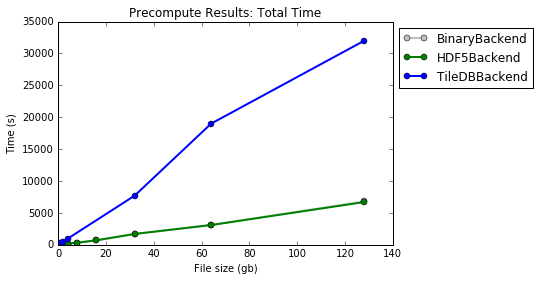
\includegraphics[scale=0.75]{./img/precompute-exp-total-time.png}
\caption{Total runtime for different backend implementations in the precompute
  experiment.}
\label{fig:precompute-exp-total-time}
\end{center}
\end{figure}

We show the total runtime of the precompute program in
Figure~\ref{fig:precompute-exp-total-time}. We can see that the total time is
dominated by reading the data, with a small amount of time for processing the
FFT across the data windows.

\subsection{Storage Overhead}

In this section we discuss the storage overhead for using each
\c{StorageBackend} type. We define this overhead as any additional disk space
required aside from the desired size of the file. As
Table~\ref{table:storage-overhead} shows, TileDB incurs a large overhead. This
overhead is primarily because of the storing the coordinate values (the $(i,j)$
coordinates within the matrix). TileDB does have some bookkeeping structures,
however these are of constant size for a given array. We allow TileDB to GZIP
the coordinate values to reduce the overhead, but there is currently no
mechanism to remove them entirely. \\

The \c{BinaryBackend} has a $0\%$ overhead because each file only has an additional
80 bytes to store the header information. Similarly, HDF5 has a small overhead,
for internal data structures describing the array.

\begin{table}[h!]
\centering
 \begin{tabular}{|c |c |c |c|}
  \hline
  \c{StorageBackend} & Max. Overhead ($\%$) & Avg. Overhead ($\%$) \\
  \hline
  \c{BinaryBackend} & $0$ & $0$ \\
  \hline
  \c{HDF5Backend} & $2.4$ & $1.5$ \\
  \hline
  \c{TileDBBackend} & $38$ & $38$ \\
  \hline
\end{tabular}
\caption{Storage overhead costs for each \c{StorageBackend} type.}
\label{table:storage-overhead}
\end{table}


\chapter{Compute Layer}\label{compute-ch}

The compute layer is responsible for two important sections of Pinky's
functionality. First, this layer handles interaction between the storage layer
by using the \c{StorageBackend} abstraction to read and write dataset and
visualization layer by performing calculations a client's request and
transferring data back for rendering. In addition, this layer also contains
implementations of optimized algorithms for processing EEG data to produce the
spectrogram visualization.

\section{Design}

Since this layer of the system supports a variety of features, we separate the
design points for each. As with other layers, minimizing runtime was one of the
key design goals, in addition to enabling developers to easily modify and add
new processing algorithms.

\subsection{Websocket Server}

The websocket server is responsible for transferring array based data to the
client for rendering. The server must be able to quickly serialize data from
the storage layer, namely multidimensional arrays of floating point values. The
server must be able to run concurrently in order to handle multiple client
requests, processing the requests in parallel to reduce latency.

\subsection{Webapp Server}

The webapp server is responsible for serving web resources such as JavaScript,
HTML, and CSS to the client. The scripts that are sent to the client are
responsible for communicating with the websocket server, retrieving data for
display. This server is separate from the websocket server to simplify the
implementation since the webapp server is not subject to the same performance
requirements when transferring datasets over the network. The separation of
these two servers allows for modules to be easily added to the webapp framework
using existing frameworks (see Section~\ref{compute-ch:implementation-webapp})
such as authentication.

\subsection{File Ingestion Daemon}

The file ingestion daemon is responsible for collecting new files that are
added to the system and converting them for use. This makes use of conversions
between the EDF format and the required format for the \c{StorageBackend} that
is in use. Input files are initially received in the EDF format and must
subsequently be converted without affecting other clients who are using the
system.

\subsection{EEG Spectrogram}\label{compute-ch:design-spectrogram}

TODO, discussing the algorithms in detail.

\section{Implementation}

The compute layer is implemented almost entirely in C++ except for the file
ingestion daemon and webapp server which are written in Python. The Python
implementations comprise a much smaller part of the compute layer codebase
since there are a number of libraries available in the community. Although
there is a cost for using multiple languages within a system, Python seemed the
appropriate choice in this circumstance due to the reduced developer time and
dependency on mature libraries. C++ was chosen for the other parts of the
module since the performance gains with a compiled language were necessary. C++
was chosen over pure C for the available libraries for linear algebra
processing \cite{arma} and network communication \cite{websocket-server}.

\subsection{Websocket Server}\label{compute-ch:implementation-ws-server}

The websocket server primarily depends on the open source library
\cite{websocket-server}. This library implements the websocket protocol and
provides a simple interface for transferring data across the network. The
library was not without problems, over the course of use we reported and helped
debug concurrency issues with the generous help of the maintainer.  These bug
fixes also resulted in large performance gains from the initial implementation
with reduced network latency. \\

When a client loads the Pinky frontend into their browser, the client sends a
request to the websocket server to open a connection. When the client wishes to
browse a patient's data, a request is send specifying the patient's \c{mrn},
the \c{channel} (LL, LP, RL, RP, see
Section~\ref{compute-ch:implementation-spectrogram}), a \c{start\_time} and
\c{end\_time} given in hours. \\

The websocket server then requests a spectrogram with the given values either
computing the spectrogram on the fly or using a precomputed spectrogram
calculation. The websocket server with potentially downsample the response to
meet client latency requirements, however, this functionality is detailed in
Chapter~\ref{visgoth-ch}. \\

To send data back to the client, a JSON encoded header is created, notifying
the client on the calculation results. The header contains a small amount of
metadata such as the sampling rate, \c{fs}, calculated \c{start\_time} and
\c{end\_time} (these values are validated to the bounds of the dataset),
spectrogram matrix dimensions and the \c{channel} the calculation was completed
for. The messaging protocal transfer binary data encoding a header length in a
\c{uint32\_t} followed by the serialized header information and the matrix data.
All messages are byte aligned to 8 bytes so a small amount of padding may be
added for performance reasons. \\

The websocket spawns $n_{processors} - 1$ threads to serve requests with. For
development and testing we have use the CSAIL OpenStack framework to create
multicore virtual machines for testing.

\subsection{Webapp Server}\label{compute-ch:implementation-webapp}

The webapp server is implemented using the Python mircoframework Flask
\cite{flask}. The Flask framework allows simple serving of HTML webpages with
support of the Jinja2 \cite{jinja2} templating system. This is vastly easier to
develop on than maintain than a comparable C++ implementation, and since
performance is not an issue it is a viable option. \\

The server provides web resources for the client as well as pages with
information about the project.

\subsection{File Ingestion Daemon}

The file ingestion daemon is implemented as a Python script that monitors the
server's filesystem for changes in order to ingest data files as they are
added. Taking advantage of the Watchdog \cite{watchdog} library, the script is
able to receive events for changes to the filesystem for a given folder. Upon
receiving a notification, the script will convert the file to the necessary
format and also precompute the spectrogram. To process the file, the script
calls the command line programs \c{edf\_converter
  <mrn>}~\ref{storage-ch:implementation-cmd} and \c{precompute\_spectrogram
  <mrn>}~\ref{compute-ch:implementation-cmd}. \\

This functionality allows an administrator to dump EDF files onto the
filesystem of the server and allow them to automatically be queried by an
analyst.

\subsection{EEG Spectrogram}\label{compute-ch:implementation-spectrogram}

The spectrogram calculation involves reading portions of the raw EEG data,
taking the FFT of the data with a sliding window in time and storing the
results in a matrix for visualization. The way the spectrogram is computed can
vary based on a number of parameters, and to simplify the implementation, we
store all relevant spectrogram parameters in an object, \c{SpecParams}. When a
client requests a spectrogram for a given region of the brain, this object is
created, building the parameters from the input \c{mrn}, \c{start\_time} and
\c{end\_time}. \\

The \c{SpecParams} object contains the following parameters, the comments next
to each parameter describe it's use.

\begin{lstlisting}
    string mrn; // patient medical record number
    StorageBackend* backend; // array storage backend
    float start_time; // start time of the spectrogram
    float end_time; // end time of spectrogram
    int start_offset; // start offset of raw data
    int end_offset; // end offset of raw data
    int spec_start_offset; // start offset of spectrogram data
    int spec_end_offset; // start offset of spectrogram data
    int fs; // sample rate
    int nfft; // number of samples for fft
    int nstep; // number of steps
    int shift; // shift size for windows
    int nsamples; // number of samples in the spectrogram
    int nblocks; // number of blocks
    int nfreqs; // number of frequencies
\end{lstlisting}

Using the \c{SpecParams} object, we can calculate the spectrogram for the EEG
data. The algorithm's pseudocode is presented below. A detailed description of
the algorithm can be found in Section~\ref{compute-ch:design-spectrogram}.

\begin{lstlisting}
void eeg_spectrogram(SpecParams* spec_params, int ch, fmat& spec_mat)
{
  // Get the column which contains the first channel for the region.
  ch_idx1 = DIFFERENCE_PAIRS[ch].ch_idx[0];
  frowvec vec1, vec2; // initialize read vectors
  read_array(mrn, ch_idx1, start_offset, end_offset, vec1);

  for (int i = 1; i < NUM_DIFFS; i++)
  {
    // Get the column which contains the next channel for the region.
    ch_idx2 = DIFFERENCE_PAIRS[ch].ch_idx[i];
    read_array(mrn, ch_idx2, start_offset, end_offset, vec2);
    // take the difference between the channel pair
    frowvec diff = vec2 - vec1;

    // fill in the spec matrix with FFT values
    FFT(spec_params, diff, spec_mat);
    swap(vec1, vec2);
  }
  spec_mat /=  (NUM_DIFFS - 1); // average diff spectrograms
  spec_mat = spec_mat.t(); // transpose the output
}
\end{lstlisting}

The definition of the constants \c{DIFFERENCE\_PAIRS} and \c{NUM\_DIFFS} are
omitted from the pseudocode for simplicity. The \c{DIFFERENCE\_PAIRS} simply
defines which channels to take differences to form a region (see
Section~\ref{compute-ch:design-spectrogram}) and \c{NUM\_DIFFS=4} since we
compute the spectrogram across four different regions of the brain. \\

The FFT algorithm is implemented using the FFTW library \cite{fftw} for optimal
performance and uses a Hanning windowing function between FFT runs. We make use
of the Armadillio C++ linear algebra library \cite{arma} for simplifying
vector/matrix calculations.

The Hamming window is defined as follows:

\begin{lstlisting}
void hamming(int windowLength, float* buf)
{
  for (int i = 0; i < windowLength; i++)
  {
    buf[i] = 0.54 - (0.46 * cos(2 * M_PI *
                    (i / ((windowLength - 1) * 1.0))));
  }
}
\end{lstlisting}

\subsection{Command Line Programs}\label{compute-ch:implementation-cmd}

The compute module offers two command line scripts, \c{test} and
\c{precompute\_spectrogram <mrn>}. The \c{test} script is used for testing new
functionality to an algorithm or \c{StorageBackend}. The
\c{precompute\_spectrogram} program will take a \c{mrn} as input and calculate
and store the spectrogram for the given \c{mrn}.

\subsection{Optimizations}

The implementation of the \c{eeg\_spectrogram} algorithm was designed with
minimizing memory consumption in mind. For this reason the \c{vec1}, \c{vec2},
and \c{spec\_mat} buffers were reused during the calculation. We considered
computing each of the differences for a region in parallel, however computing
each region in parallel (parallelized at the websocket server) was performant
enough. Previous iterations involved serializing the output of the Armadillio
matrix (\c{fmat}), however we found that instead we could directly access a
pointer of the raw buffer memory. This optimization help significantly since it
eliminated a memory allocation and data copying before sending over the
network. \\

Another minor optimization is the use of the \c{static inline} keyword. We use
this for helper functions to reduce function call overhead. In addition, we
always pass Aramdillo objects by reference and not value, avoiding a copy on
function calls.

\section{Related Work}


\chapter{Visualization Layer}\label{viz-ch}

The primary function of the visualization layer is to render a spectrogram
served by the compute layer. In addition, this module is responsible for
providing a usable interface for an analyst to work with the datasets.
Minimizing latency is an important design goal since increased latency can
dramatically reduce an analyst's efficiency if they must continually wait for
the interface to respond to queries. \\

We chose to build browser based visualizations to simplify the use for an
analyst -- the only software required is the browser itself. In addition, the
analyst does not require special hardware since the server handles the
intensive storage and computations.  This choice makes the job of visualizing
interactively more difficult since the browser is much more limited in network
bandwidth and rendering capabilities compared to a native application.

\section{Design}

\subsection{Interface}

The interface should provide the analyst with the ability to specify a patient
\c{mrn} to query, a \c{start\_time} and \c{end\_time} and also afford quick
navigation between time ranges. The workflow that we anticipate is that an
analyst will load a single patient file and browse subsequent time frames. Upon
reaching a section of interest, the analyst should be able to zoom in to see
further details. The interface should also give the analyst information about
the visualization, such as interactive axes. The interface should also provide
user feedback for errors, cleaning data on the client to prevent the
inadvertent issuing of queries.

\subsection{Communication}

Optimizing communication is important to avoid creating a bottleneck that can
affect latency. The point which is most likely to be a bottleneck is
deserializing the data received from the network.

\subsection{Rendering}

The client rendering must be able to efficiently render large matrices of
floating point values, on the order of several million points. The spectrogram
visualization is created by taking the intensity of the $(i, j)$-th entry in
the spectrogram and mapping it to a rendered color in the $(i, j)$-th pixel on
screen. Some amount of data aggregation is acceptable, for example
downsampling, however the analyst must not experience degradation of the
overall data quality. \\

\section{Implementation}

We implement the visualization layer primarily using HTML, JavaScript and CSS.
WebGL performs the rendering to take advantage of a client's GPU.

\subsection{Interface}

Figure~\ref{fig:whole-interface} shows the implementation of the interface. The
interface shows a sample of a patient with \c{mrn} `\c{005}' rendered between
the second and third hour of the scan. These parameters are located in the top
bar, in addition to controls which enable the analyst to scroll to previous or
next hour with a single click. The scrolling interval defaults to 1 hour, but
is configurable in the settings window. \\

\begin{figure}[h]
\begin{center}
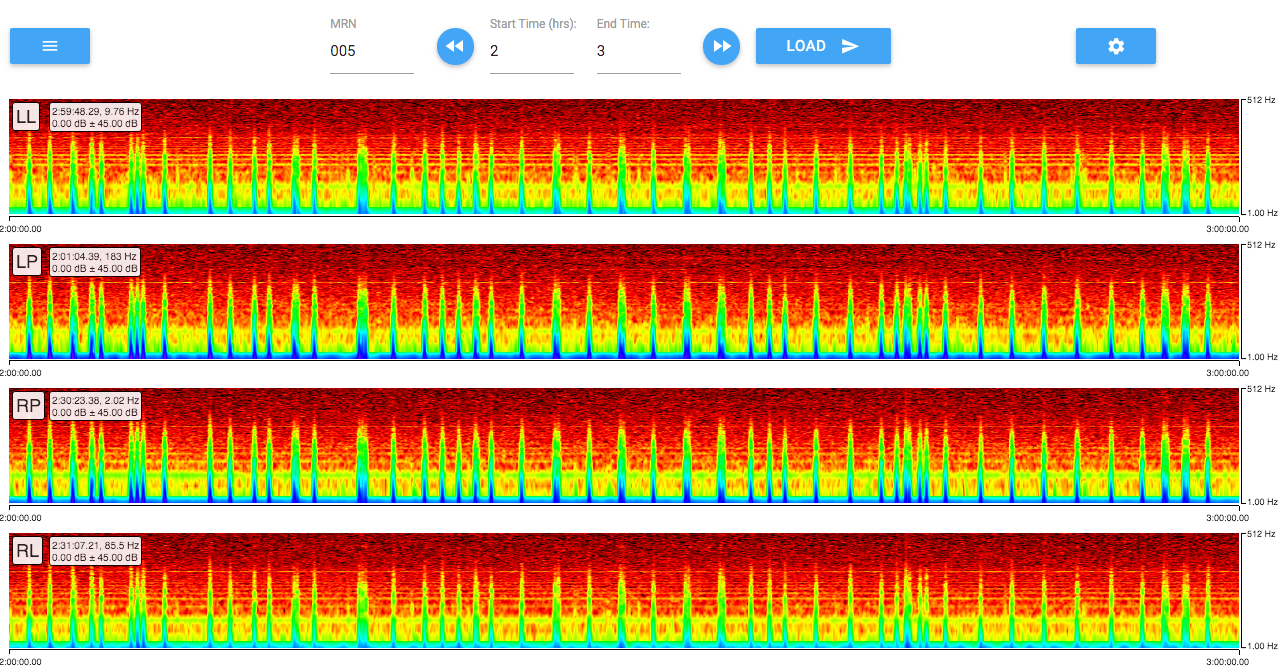
\includegraphics[scale=0.35]{./img/whole-interface.png}
\caption{Screenshot of Pinky's user interface.}
\label{fig:whole-interface}
\end{center}
\end{figure}

Clicking the the small gear on the far right of the interface opens the
settings page, the available options are shown in Figure~\ref{fig:settings}.
The settings page allows an analyst to change the rendering mode, time interval
and select options for interpolation and the visualization scale. In addition,
there are two keyboard shortcuts which allow an analyst to change the amplitude
scale or zoom in on the visualization. Figure~\ref{fig:zoomed-region} shows the
result of a single region when a user has zoomed in. \\

\begin{figure}[h]
\begin{center}
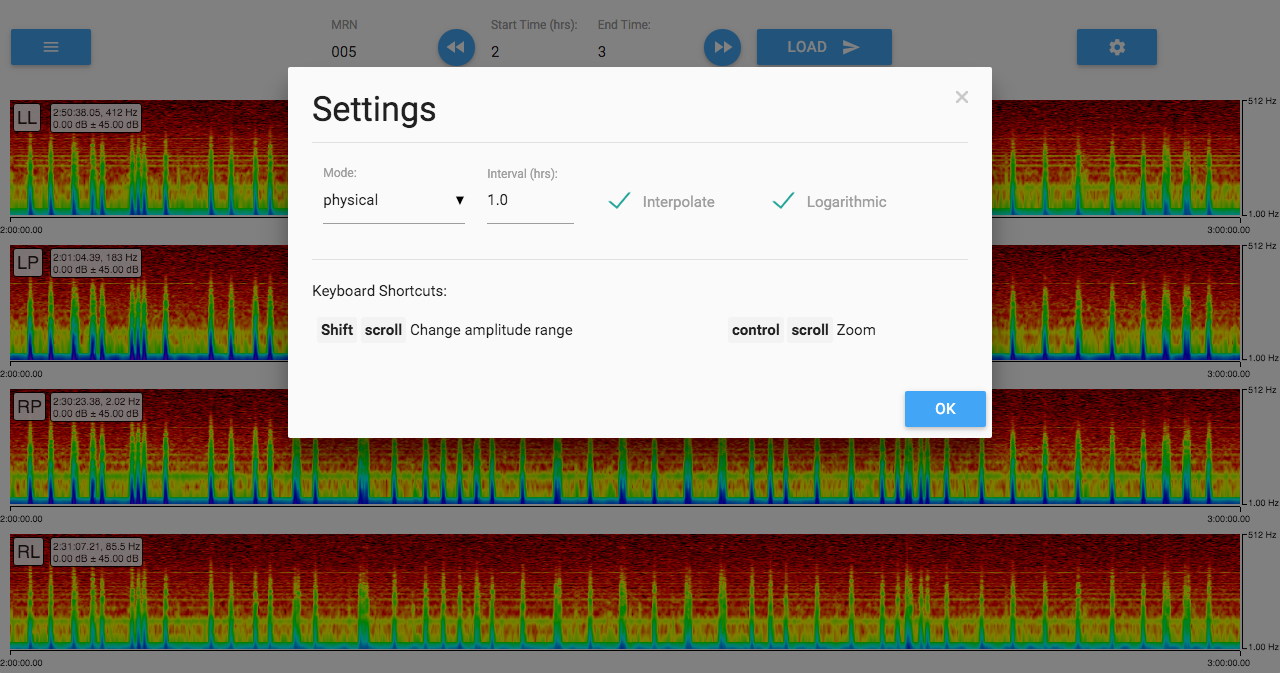
\includegraphics[scale=0.35]{./img/settings.png}
\caption{Screenshot of the settings modal.}
\label{fig:settings}
\end{center}
\end{figure}

The interface shows a spectrogram for each region of the brain, each region is
label in the upper left hand corner with \c{LL}, \c{LP}, \c{RP}, or \c{RL}.  As
Figure~\ref{fig:zoomed-region} shows, next to these labels, is a small box
containing axis information, specifying where the user's mouse currently is. In
this box the current timestamp (x-axis) and frequency (y-axis) are show. In
addition, the box shows the current amplitude value in dB and the current
amplitude viewing range. \\

\begin{figure}[h]
\begin{center}
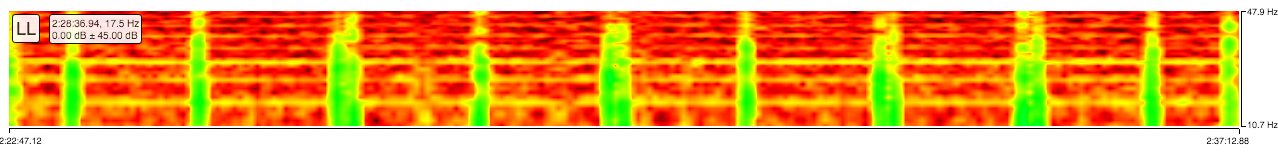
\includegraphics[scale=0.35]{./img/zoomed-region.png}
\caption{Screenshot of a zoomed spectrogram view of a single rendered region
  with dynamic axis labels.}
\label{fig:zoomed-region}
\end{center}
\end{figure}

While loading, the interface blurs the spectrograms and presents a loading bar
to the user, as shown in Figure~\ref{fig:loading}. A delay between the
rendering of each region can cause confusion about the current rendered data.
Blurring a region and placing a loading bar on it clearly shows the new region
has not yet updated to the client's latest query. \\

\begin{figure}[h]
\begin{center}
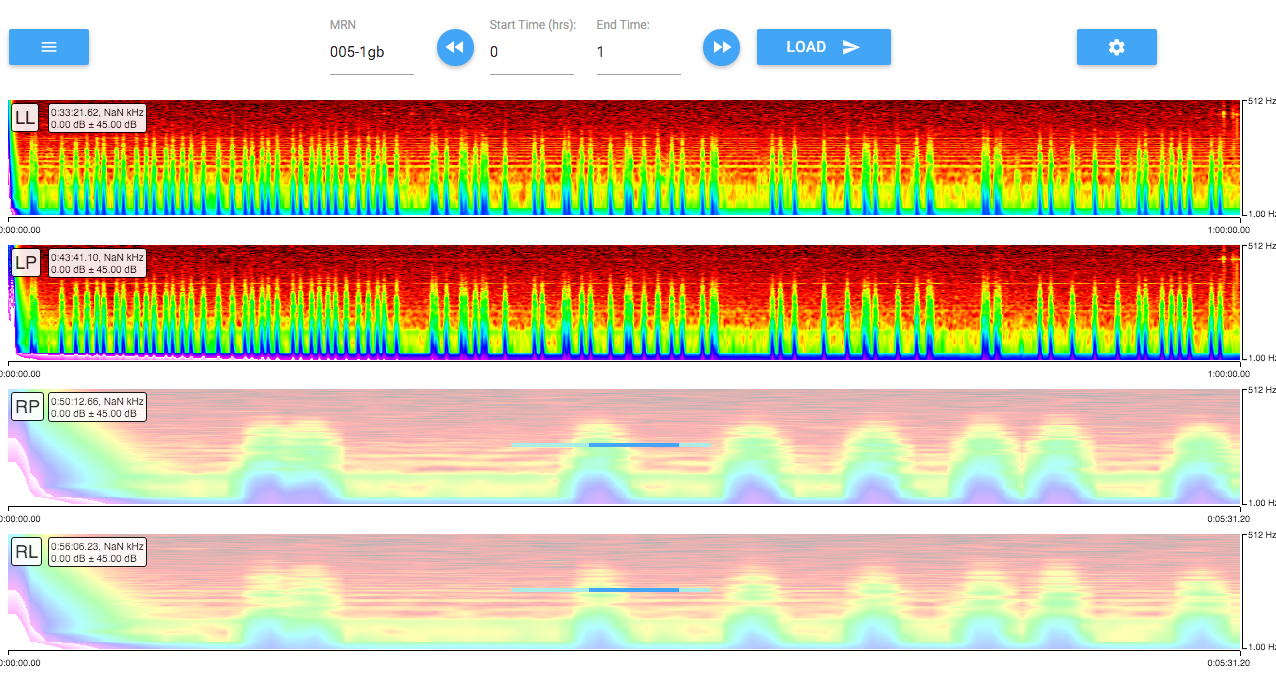
\includegraphics[scale=0.35]{./img/loading.png}
\caption{Screenshot of loading interface.}
\label{fig:loading}
\end{center}
\end{figure}

If an analyst enters an invalid \c{mrn}, the interface responds by clearing all
of the rendered spectrograms and displaying a small error message, shown in
Figure~\ref{fig:error}. An invalid \c{mrn} is simply one which the
\c{StorageBackend} does not contain an array for. This could be from a user slip
error or if the system is currently ingesting the array. This user interaction
is important to avoid analyst confusion when issuing an invalid query. \\

\begin{figure}[h]
\begin{center}
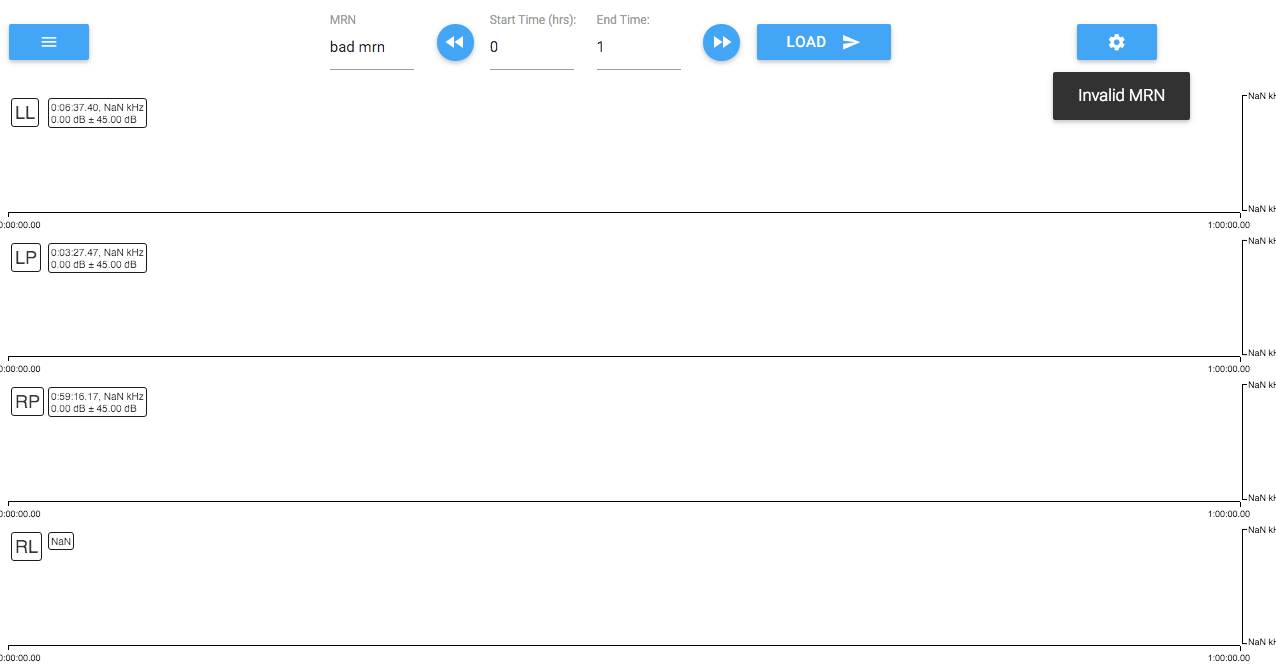
\includegraphics[scale=0.35]{./img/error.png}
\caption{Screenshot of invalid \c{mrn} error message.}
\label{fig:error}
\end{center}
\end{figure}

The CSS library Materialize \cite{materialize} was used to layout the page
structure and keep a consistent style throughout the webapp.

\subsection{Communication}

A websocket communicates with the compute layer websocket server using a binary
protocol described in Section~\ref{compute-ch:implementation-ws-server}. We
send requests as JSON encoded data and receive binary responses containing the
computed spectrogram data for a given region.

We make use of the reconnecting-websocket \cite{reconnecting-websocket} library
to ensure a smooth user experience if the analyst does not use the page and the
connection to closes. This library automatically reopens the connection,
instead of forcing the analyst to refresh the page altogether.

\subsection{Rendering}

WebGL is a JavaScript API which can render interactive 2D or 3D computer
graphics without the use of any third party plugins. The initial implementation
used the open-source library WebGL-Spectrogram \cite{webgl-spectrogram}. This
library has the functionality to render the spectrogram of an audio file using a
lightweight Python websocket server. We modified this library to a more general
version to contain multiple canvases, one for each brain region, and to
communicate with the compute layer websocket server. \\

\subsection{Optimizations}

WebGL was chosen since it is much more performant than using a browser's canvas
object or rendering DOM elements directly. Each spectrogram is an array on the
order of millions of points, we would not be able to achieve the latency
required for interactivity without the GPU rendering. Development time suffers
from the use of WebGL since it is difficult to understand the programming model
without some background in graphics rendering. In addition, we use JavaScript
typed arrays to transfer the binary data from the websocket to the GPU.
JavaScript typed arrays are array-like objects providing access raw binary
data. JavaScript engines optimize these arrays giving higher performance than
the traditional JavaScript \c{Array} object.


\chapter{Visgoth System}\label{visgoth-ch}

The Visgoth system is responsible for monitoring client and server performance
statistics to ensure that a certain latency is met. Using an experimental
model, the system can reduce the granularity of the data delivered to the
client in an attempt to reduce latency. The system aims at using the collected
statistics to adapt to client or server load by aggregating the visualization,
reducing the overall data that must be transferred and rendered by the client. \\

\section{Design}
\section{Implementation}
\section{Related Work}
\section{Evaluation}

\appendix
\chapter{Tables}

\begin{table}
\caption{Armadillos}
\label{arm:table}
\begin{center}
\begin{tabular}{||l|l||}\hline
Armadillos & are \\\hline
our	   & friends \\\hline
\end{tabular}
\end{center}
\end{table}

\clearpage
\newpage

\chapter{Figures}

\vspace*{-3in}

\begin{figure}
\vspace{2.4in}
\caption{Armadillo slaying lawyer.}
\label{arm:fig1}
\end{figure}
\clearpage
\newpage

\begin{figure}
\vspace{2.4in}
\caption{Armadillo eradicating national debt.}
\label{arm:fig2}
\end{figure}
\clearpage
\newpage

%% This defines the bibliography file (main.bib) and the bibliography style.
%% If you want to create a bibliography file by hand, change the contents of
%% this file to a `thebibliography' environment.  For more information 
%% see section 4.3 of the LaTeX manual.
\begin{singlespace}
\bibliography{main}
\bibliographystyle{plain}
\end{singlespace}

\end{document}

